\documentclass[a4paper,10pt]{jsarticle}

% 数式
\usepackage{amsmath,amsfonts}
\usepackage{bm}
% 画像
\usepackage[dvipdfmx]{graphicx}

\usepackage{listingsutf8,jlisting} %日本語のコメントアウトをする場合jlistingが必要
%ここからソースコードの表示に関する設定
\lstset{
  basicstyle={\ttfamily},
  identifierstyle={\small},
  commentstyle={\smallitshape},
  keywordstyle={\small\bfseries},
  ndkeywordstyle={\small},
  stringstyle={\small\ttfamily},
  frame={tb},
  breaklines=true,
  columns=[l]{fullflexible},
  numbers=left,
  xrightmargin=0zw,
  xleftmargin=3zw,
  numberstyle={\scriptsize},
  stepnumber=1,
  numbersep=1zw,
  lineskip=-0.5ex
}

\begin{document}

\title{ソフトウェア設計法レポート第3回}
\author{坪井正太郎(101830245)}
\date{\today}
\maketitle
\section{システム境界}
\begin{figure}[htb]
  \centering
  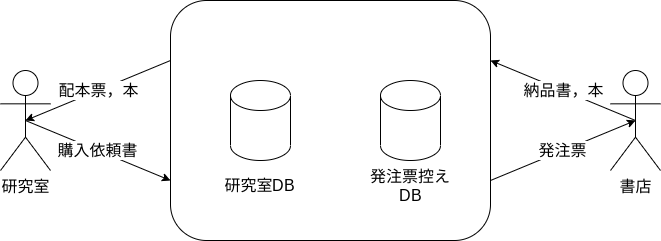
\includegraphics[width=\linewidth]{./01.png}
\end{figure}

\section{構成要素}
構成要素は以下のようになる。
\begin{itemize}
  \item 研究室
  \item 書店
  \item 研究室DB
  \item 発注票控えDB
  \item 購入依頼書の処理
  \item 発注票の作成,発注
  \item 納品書,本の処理
  \item 配本票の作成,配布
\end{itemize}

\section{構成要素間の関係}
\begin{itemize}
  \item \textbf{(購入依頼書の処理)研究室は,図書館に購入依頼書を提出する。購入依頼書は,書名,価格,研究室を含む。}\\図書館は,研究室DBから予算残高と支出予定額を取得し,支出予定額との合計が予算残高を超えないか調べる。\\超えないならば,(発注票の作成,発注)に書名,価格,研究室の情報を伝える。\\

  \item \textbf{(発注票の作成,発注)図書館は,伝えられた情報から発注票とその控えを作成する。発注票は書名,価格,発注者名,発注番号,発注日,の情報を持つ。}\\図書館は,研究室DBの支出予定額を発注表の価格分だけ増やす。控えは,控えDBに保存される。図書館は,作成した発注票を書店に提出する\\

  \item \textbf{(納品書,本の処理)書店は,図書館に納品書と本を届ける。図書館は,書店から納品書と本が届けられると,納品書の処理を行う。納品書は書名,価格,発注番号,の情報を含む。}\\図書館は,発注票控えDBに同じ発注番号を持つ発注票控えがあれば,納品書を受理する。受理するならば,研究室DBの該当研究室の予算残高を,納品書にある価格分減らす。同時に,発注票控えにある価格分の支出予定額を減らす。\\(配本票の作成)に書名,価格,発注書控えの研究室名,の情報を伝える。\\

  \item \textbf{(配本票の作成)図書館は,伝えられた情報から,配本票を作成する。配本票は書名,価格,研究室名,の情報を持つ。}\\作成した配本票は,本とともに配本票の研究室名に対応する研究室に配布される。
\end{itemize}

\end{document}
